 \documentclass{article}
 \usepackage{graphicx}
 \graphicspath{ {./images/} }
 
 \usepackage{hyperref}
 \hypersetup{
    colorlinks=true,
    linkcolor=blue,
    filecolor=magenta,      
    urlcolor=cyan,
 }

 \usepackage{parskip}
 \usepackage{amsmath}
 
 \begin{document}
 
 \begin{center}
     \Huge\textbf{Homework 4: Sukrit Ganesh}\par
 \end{center}
 
  \noindent\makebox[\linewidth]{\rule{\paperwidth}{0.4pt}}\newline
 
 \begin{center}
      \Large\textbf{Problem 1:} Define a random variable X by the following procedure. Draw a card from a standard deck of playing cards. If the card is knave, queen, or king, then X = 11. If the card is an ace, then X = 1; otherwise, X is the number of the card (i.e. two through ten). Now define a second random variable Y by the following procedure. When you evaluate X, you look at the color of the card. If the card is red, then Y = X - 1; otherwise, Y = X + 1. \par
 \end{center}
 
 \textbf{Part A: | What is $P(\{X \leq 2\})$?}\newline
 
 Because the two events $X=1$ and $X=2$ are disjoint (a card cannot have the value 1 and 2), we can find P(\{$X \leq 2$\}) via the following sum: $P(\{X = 1\}) + P(\{X = 2\})$. Because this is a standard deck of cards, $P(\{X = 1\}) = \frac{4}{52}$ and $(\{X = 2\}) = \frac{4}{52}$. Hence, we find that $P(\{X \leq 2\}) = \frac{8}{52} = \frac{2}{13}$.\newline
 
 Final Answer: $\frac{2}{13}$.\newline
 
 \textbf{Part A: | What is $P(\{X \geq 10\})$?}\newline
 
 Because the two events $X=10$ and $X=11$ are disjoint (a card cannot be a face-card and a 10), we can find P(\{$X \geq 10$\}) via the following sum: $P(\{X = 10\}) + P(\{X = 11\})$. Because this is a standard deck of cards, $P(\{X = 10\}) = \frac{4}{52}$ and $(\{X = 11\}) = \frac{12}{52}$. Hence, we find that $P(\{X \leq 2\}) = \frac{16}{52} = \frac{4}{13}$.\newline
 
 Final Answer: $\frac{4}{13}$.\newline
 
 \textbf{Part C: | What is $P(\{X \geq Y\})$?}\newline
 
 We are given that $Y = X - 1$ when the drawn card is red and $Y = X + 1$ when the card is black. We can rearrange the equations to get the following: $X = Y + 1$ when the drawn card is red and $X = Y - 1$ when the card is black. Clearly, $X \geq Y$ only when the drawn card is red, because $X < Y$ when the card is black. The probability that the drawn card is red, and subsequently the probability that $X \geq Y$, is $\frac{1}{2}$.\newline
 
 Final Answer: $\frac{1}{2}$.\newline
 
 \textbf{Part D: | What is the probability distribution of $Y-X$?}\newline
 
 We are given that $Y = X - 1$ when the drawn card is red and $Y = X + 1$ when the card is black. Hence, $Y-X = (X-1)-X=-1$ when the drawn card is red and $X-Y=(X+1)-X=1$ when the card us black. Because $P(red card) = \frac{1}{2} and P(black card) = \frac{1}{2}$, the discrete probability distribution of $Y-X$ will look like the following: \newline
 
 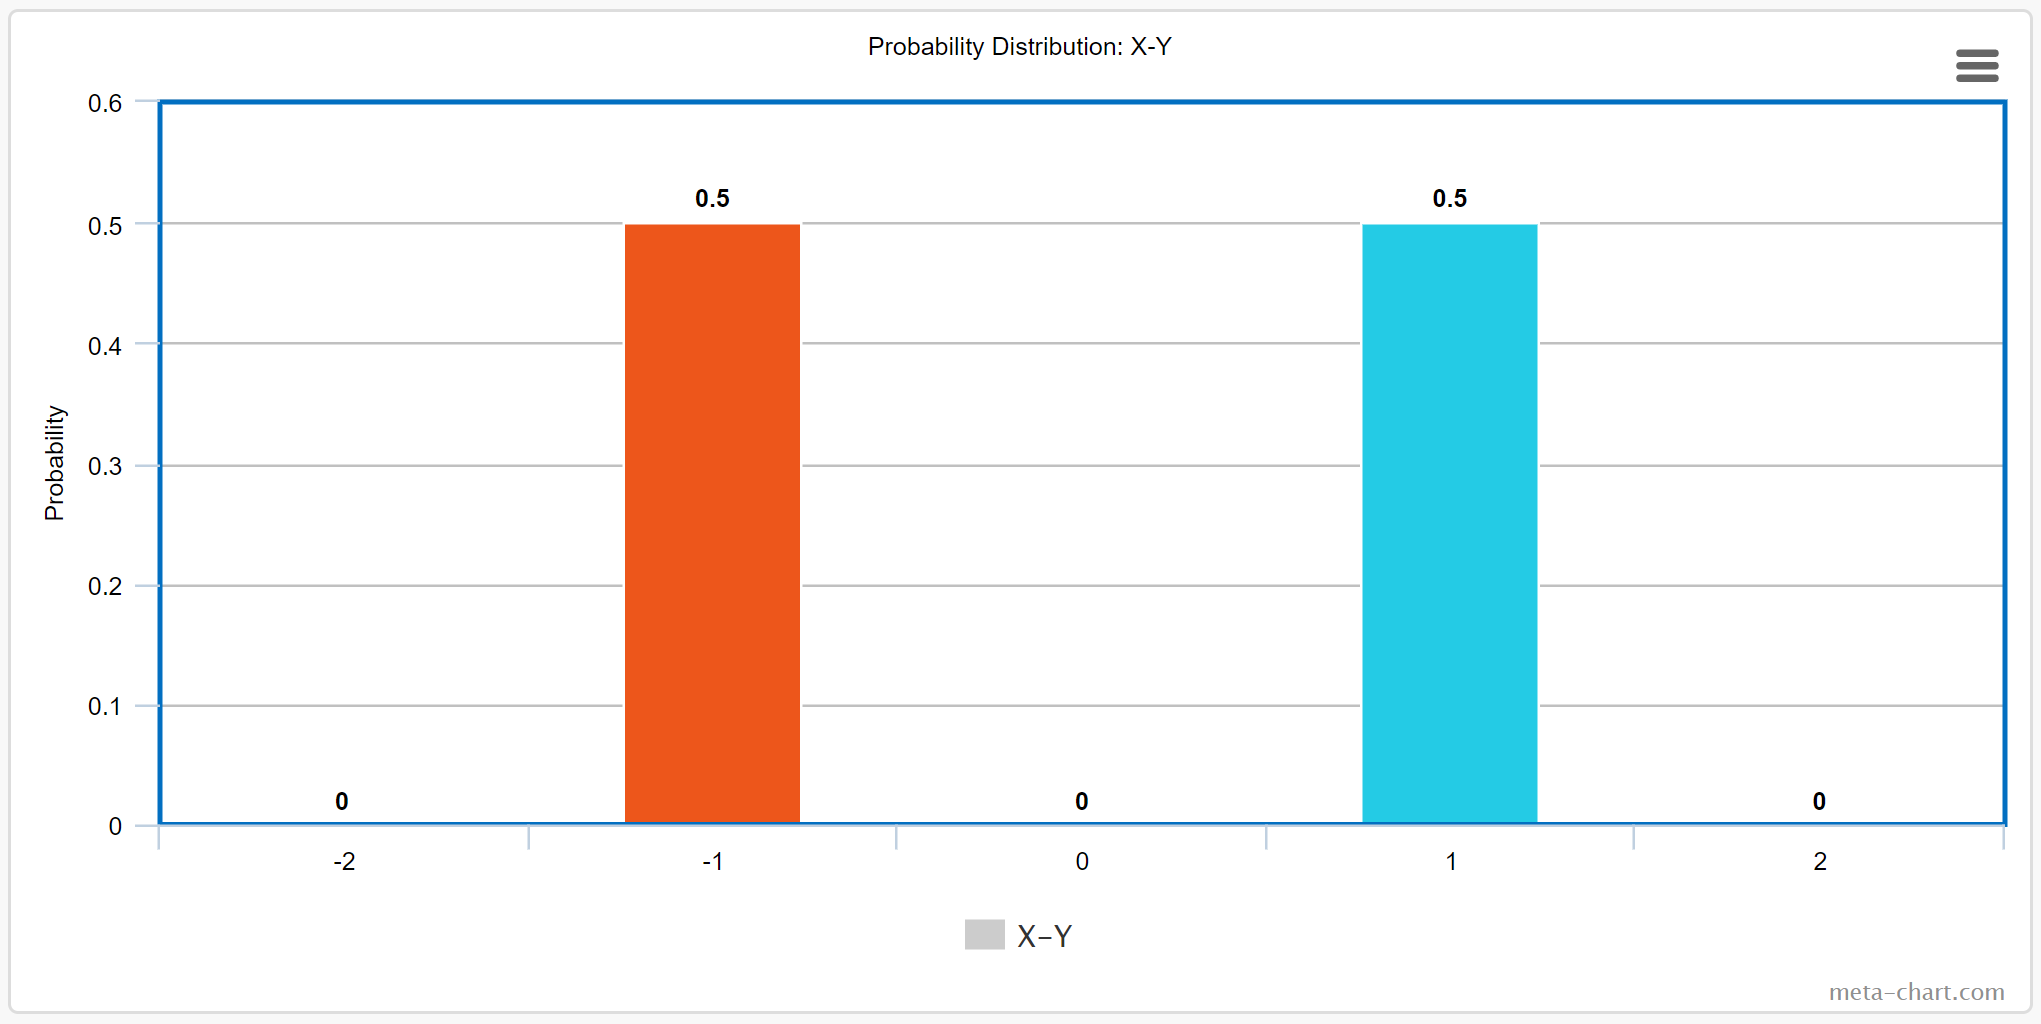
\includegraphics[scale=0.565]{HW4_1.PNG}
 
 The probability distribution can also be expressed as a piecewise function:
 
 \begin{displaymath}
    P(Y-X)=
    \begin{cases} 
        0.5 & x = -1 \\
        0.5 & x = 1 \\
        0 & otherwise
    \end{cases}
 \end{displaymath}
  
 \textbf{Part E: | What is $P(\{Y \geq 12\})$?}\newline
 
 We are given that $Y=X+1$ if the drawn card is black. Because X can be at most 11 (when a face card is drawn), Y can be at most 12, which happens when a black face card is drawn. Y is at most 10 when a red card is drawn, because in that case, $Y=X-1$. The probability of drawing a black face card is the product of the probability of drawing a black card and the probability of drawing a face card, since the two events are independent. Hence, we find that $P(\{Y \geq 12\}) = P(black card) * P(X=11) = \frac{1}{2} * \frac{12}{52} = \frac{6}{52} = \frac{3}{26}$.\newline
 
 Final Answer: $\frac{3}{26}$.\newline
 
 \newpage
 
 \noindent\makebox[\linewidth]{\rule{\paperwidth}{0.4pt}}\newline
 
 \begin{center}
      \Large\textbf{Problem 2:} Magic the Gathering is a popular card game. Cards can be land cards, or other cards. We consider a game with two players. Each player has a deck of 40 cards. Each player shuffles their deck, then deals seven cards, called their hand. The rest of each player’s deck is called their library. Assume that player one has 10 land cards in their deck and player two has 20. Write $L_1$ for the number of lands in player one’s hand and$L_2$ for the number of lands in player two’s hand. Write $L_t$ for the number of lands in the top 10 cards of player one’s library.\par
 \end{center}
 
 \textbf{Part A: | Write $S = L_1 + L_2$. What is $P(\{S=0\})$?}\newline
 
 If $S=0$, $L_1 = L_2 = 0$. By this definition, both players' hands must be completely devoid of land cards. We can multiply $P(L_1=0)$ by $P(L_2=0)$ to find $P(L_1=0, L_2=0)$ because the two events are independent. To calculate the two probabilities, we must probabilities that 7 drawn cards without replacement are all NOT land cards for both players.
 
 \begin{displaymath}
    P(L_1 = 0) = \frac{30}{40}*\frac{29}{39}*\frac{28}{38}*\frac{27}{37}*\frac{26}{36}*\frac{25}{35}*\frac{24}{34} = 0.109 = 10.9\%.
 \end{displaymath}
 
 \begin{displaymath}
    P(L_2 = 0) = \frac{20}{40}*\frac{19}{39}*\frac{18}{38}*\frac{17}{37}*\frac{16}{36}*\frac{15}{35}*\frac{14}{34} = 0.00416 = 0.42\%.
 \end{displaymath}
 
 \begin{displaymath}
    P(L_1 = 0, L_2 = 0) = P(L_1)*P(L_2) = 0.109 * 0.00416 = 0.000454 = 0.0454\%.
 \end{displaymath}
 
 Final Answer: $0.000454 = 0.0454\%$.\newline
 
 \textbf{Part B: | Write $D = L_1 - L_2$. What is $P(\{D=0\})$?}\newline
 
 Because $D = L_1 - L_2 = 0$, $L_1 = L_2$, meaning that both players must have the same number of land cards in their hands. We will calculate the total probability by summing the probabilities that both players have 0, 1, 2, 3, 4, 5, 6, and 7 lands.\newline
 
 Once again, the probability that both players have $N$ lands - $P(L_1=N,L_2=N)$ - is simply $P(L_1)*P(L_2)$ because the two aforementioned events are independent. Additionally, because the probabilities $P(L_1=N,L_2=N)$ are disjoint, we can simply sum up the probabilities using the formula $\sum_{N=0}^{7}P(L_1=N,L_2=N)$ to find the probability that the two players have the same number of lands in their hand (ranging from 0 to 7 lands, of course, because the size of the hand is 7).\newline
 
 We can find $P(L_1=N) and P(L_2=N)$ by dividing the number of combinations which result in a hand with N lands by the total number of combinations of hands.
 
 \begin{displaymath}
    P(L_1=N)=\frac{{10 \choose N}*{30 \choose 7-N}}{{40 \choose 7}};    P(L_2=N)=\frac{{20 \choose N}*{20 \choose 7-N}}{{40 \choose 7}}
 \end{displaymath}
 
 \begin{displaymath}
    P(L_1=N, L_2=N)=P(L_1=N)*P(L_2=N)=\frac{{20 \choose N}*{20 \choose 7-N}*{10 \choose N}*{30 \choose 7-N}}{{40 \choose 7}^2}
 \end{displaymath}
 
 We can sum up the above probabilities from N = 0 to N = 7 to find $P(D=0)$.
 
 \begin{displaymath}
    P(D=0) = \sum_{N=0}^{7}\frac{{20 \choose N}*{20 \choose 7-N}*{10 \choose N}*{30 \choose 7-N}}{{40 \choose 7}^2}
 \end{displaymath}
 
 Final Answer: $\sum_{N=0}^{7}\frac{{20 \choose N}*{20 \choose 7-N}*{10 \choose N}*{30 \choose 7-N}}{{40 \choose 7}^2}$.\newline
 
 \textbf{Part C: | What is the probability distribution for $L_1$?}\newline
 
 Player 1 can have between 0 and 7 lands. $P(L_1=N)$ is calculated using the following formula: $\frac{{10 \choose N}*{30 \choose 7-N}}{{40 \choose 7}}$. \newline
 
 In order to plot the probability distribution, we must first find the individual probabilities $P(L_1=N)$ from N = 0 to N = 7. Because $0 \leq N \leq 7$, and the probabilities are disjoint, the sum of $P(L_1=N)$ from N = 0 to N = 7 must equal 1.
 
 \[P(L_1=0)=\frac{{10 \choose 0}*{30 \choose 7}}{{40 \choose 7}}=0.109\]
 \[P(L_1=1)=\frac{{10 \choose 1}*{30 \choose 6}}{{40 \choose 7}}=0.318\]
 \[P(L_1=2)=\frac{{10 \choose 2}*{30 \choose 5}}{{40 \choose 7}}=0.344\]
 \[P(L_1=3)=\frac{{10 \choose 3}*{30 \choose 4}}{{40 \choose 7}}=0.176\]
 \[P(L_1=4)=\frac{{10 \choose 4}*{30 \choose 3}}{{40 \choose 7}}=0.0457\]
 \[P(L_1=5)=\frac{{10 \choose 5}*{30 \choose 2}}{{40 \choose 7}}=0.00588\]
 \[P(L_1=6)=\frac{{10 \choose 6}*{30 \choose 1}}{{40 \choose 7}}=0.000338\]
 \[P(L_1=7)=\frac{{10 \choose 7}*{30 \choose 0}}{{40 \choose 7}}=0.00000644\]
 
 We can then plot the probability distribution.
 
 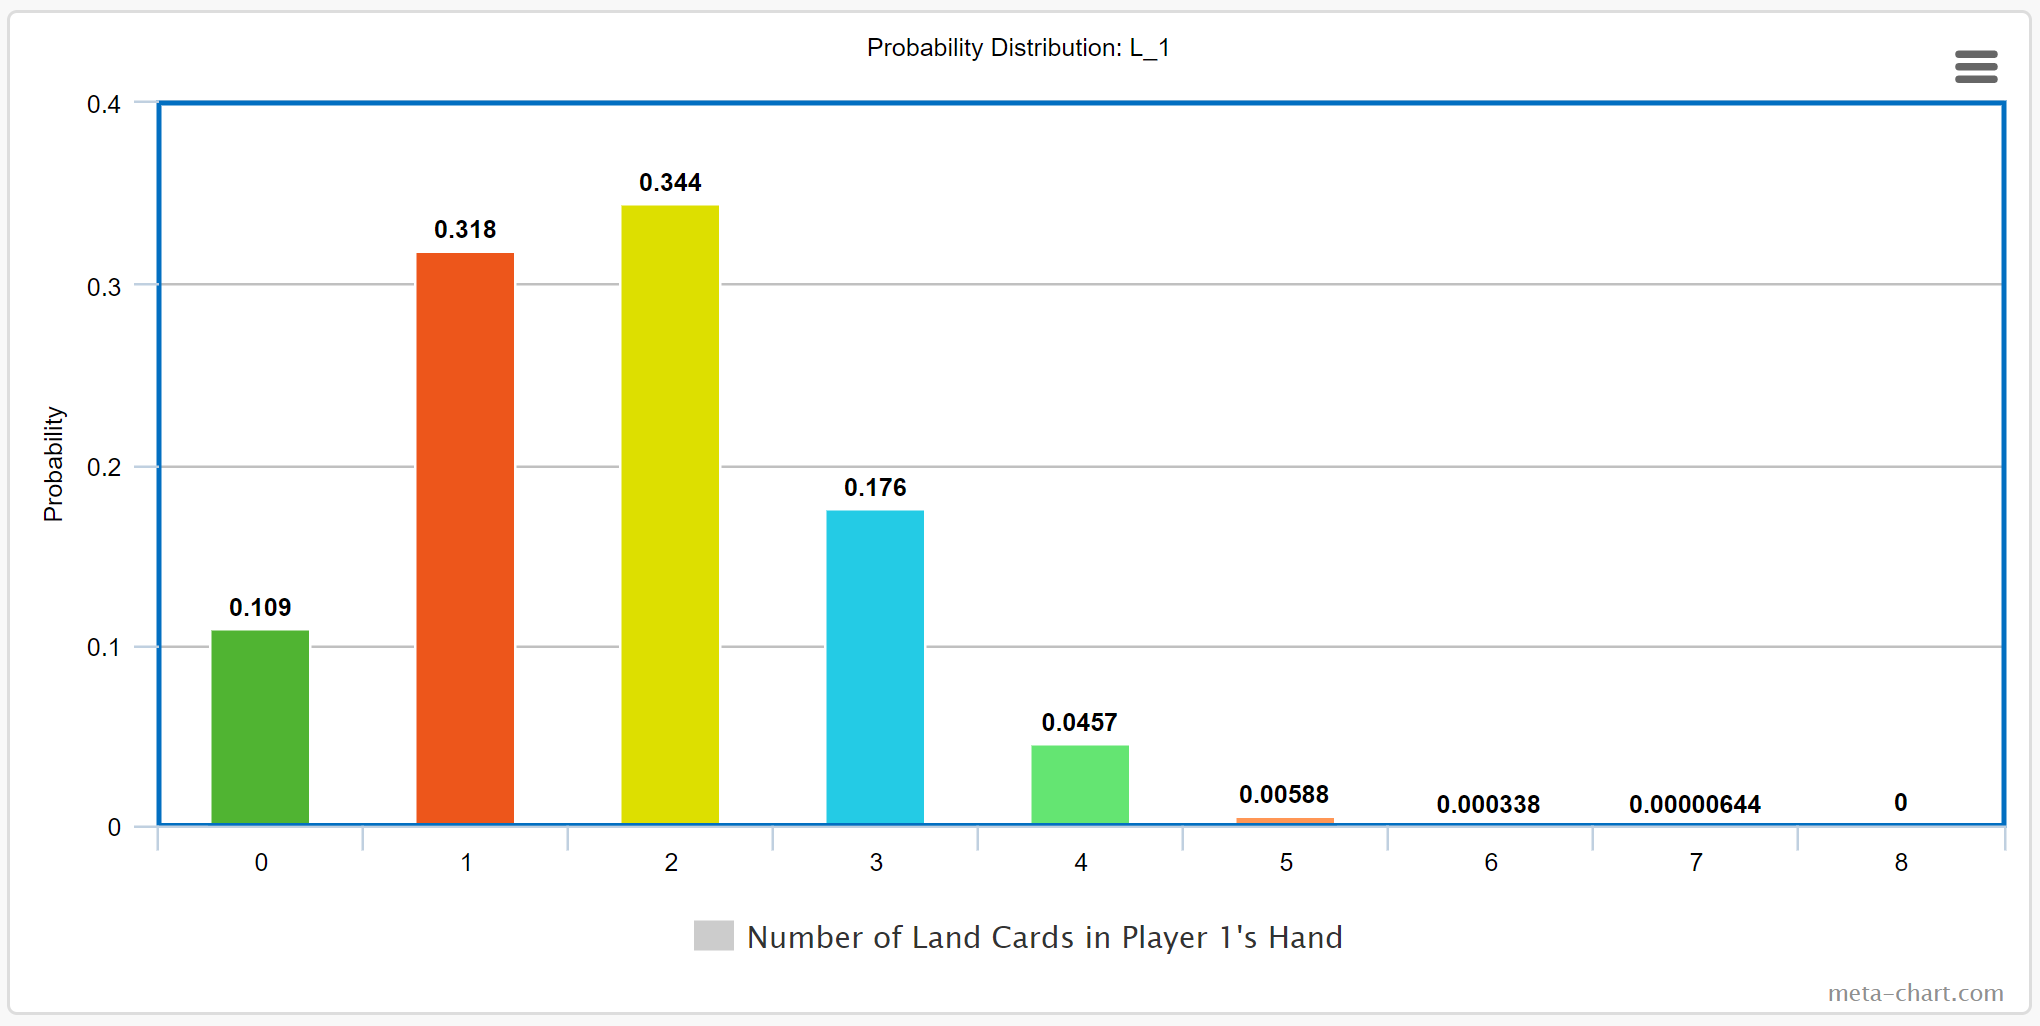
\includegraphics[scale=0.565]{HW4_2.PNG}
 
 The probability of having no land cards is lower than the probability of having 1 land card, so $P(L_1=N)$ will initially increase. However, the probabilities decline after $L_1=3$, because getting a high amount of land cards becomes harder and harder. Interestingly, more than 60\% of the time, Player 1 will have either 1 or 2 land cards. This discrete probability distribution is certainly right-skewed!\newline
 
  \textbf{Part D: | Write out the probability distribution for $P(L_1|L_t=10)$?}\newline
 
 Player 1's deck contains 10 land cards and 30 non-land cards. If the top 10 cards in the library (the 33 cards not part of the hand) contains 10 lands, then the deck MUST contain 0 lands, because all of Player 1's lands are in the library and cannot be in the hand. Mathematically, this means that $L_1=0$ if $L_t=10$. The probability distribution of $L_1$ given $L_t=10$ is not a very interesting one: the probability that $L_t = 0$ is 1, and the probability that $L_t$ equals anything else is 0. 
 
 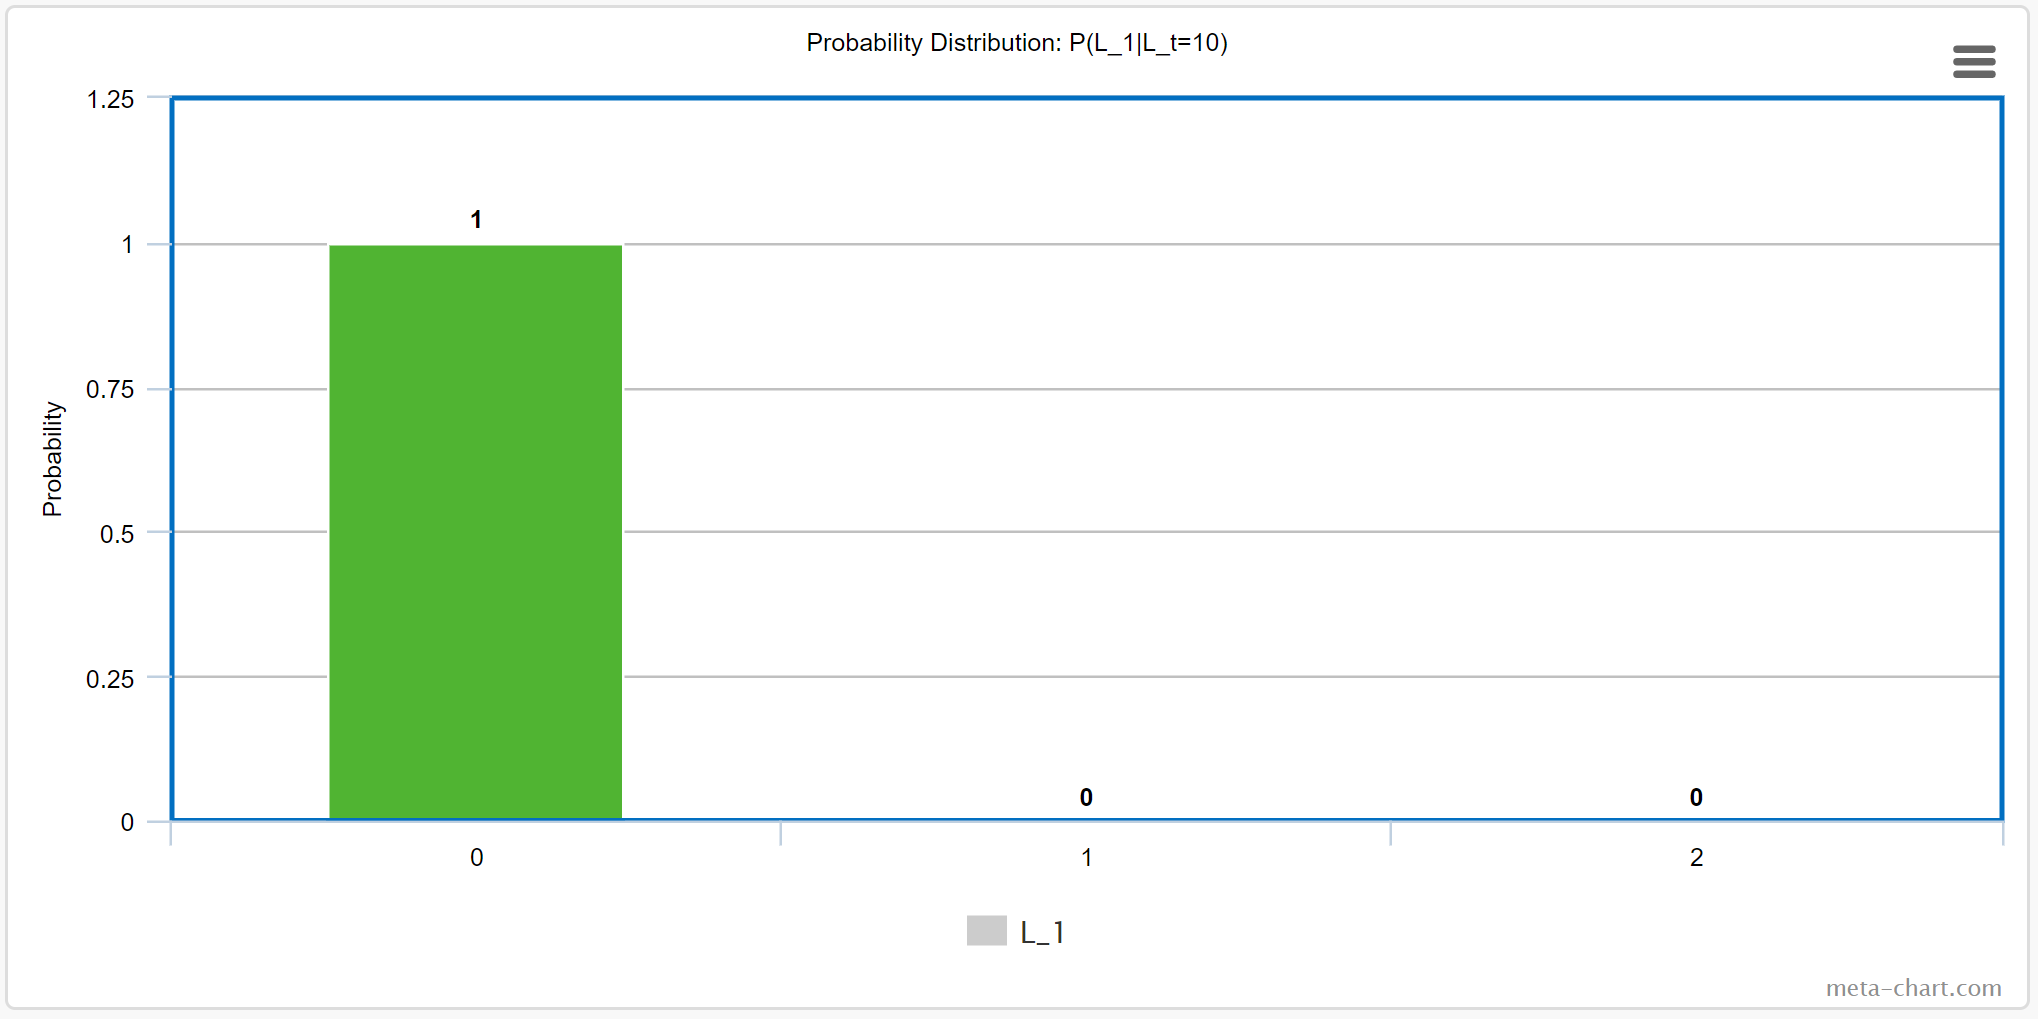
\includegraphics[scale=0.565]{HW4_3.PNG}\newline
 
 P(L_1|L_t=0)=
    \begin{cases} 
        1 & x = 0 \\
        0 & otherwise
    \end{cases}\newline
 
 \textbf{Part E: | Write out the probability distribution for $P(L_1|L_t=5)$?}\newline
 
 Player 1's deck contains 10 land cards and 30 non-land cards. If the top 10 cards in the library (the 33 cards not part of the hand) contains 5 lands, then the deck MUST contain AT MOST 5 lands. This makes intuitive sense, because if the deck has 10 lands, and 5 of those hands are definitely in the library, then the hand can have at most 5 lands. Of course, it is possible that the rest of the library (we only know the top 10 cards) contains more lands, so it is entirely possible that the player's hand contains less than 5 lands. However, 5 lands is the definite maximum for the hand. 
 
 We must calculate the probability that $L_1=N$, $N$ being the number of lands in the player's hand with $0 \leq N \leq 5$. Because 10 cards (5 lands and 5 non-lands) are KNOWN to be in the library, we have only 30 cards to choose our deck from. Seven will be in the deck, and the remaining 23 will stay in the library. We must choose $N$ land cards from 
 
 \begin{displaymath}
    P(L_1=N|L_t=5)=\frac{{5 \choose N}*{25 \choose 7-N}}{{30 \choose 7}}
 \end{displaymath}
 
 We can write out the individual probabilities, which obviously sum up to 1, as follows:
 
 \[P(L_1=0|L_t=5)=\frac{{5 \choose 0}*{25 \choose 7}}{{30 \choose 7}}=0.236\]
 \[P(L_1=1|L_t=5)=\frac{{5 \choose 1}*{25 \choose 6}}{{30 \choose 7}}=0.435\]
 \[P(L_1=2|L_t=5)=\frac{{5 \choose 2}*{25 \choose 5}}{{30 \choose 7}}=0.261\]
 \[P(L_1=3|L_t=5)=\frac{{5 \choose 3}*{25 \choose 4}}{{30 \choose 7}}=0.0621\]
 \[P(L_1=4|L_t=5)=\frac{{5 \choose 4}*{25 \choose 3}}{{30 \choose 7}}=0.00565\]
 \[P(L_1=5|L_t=5)=\frac{{5 \choose 5}*{25 \choose 2}}{{30 \choose 7}}=0.000147\]
 
 We can then plot the probability distribution.

 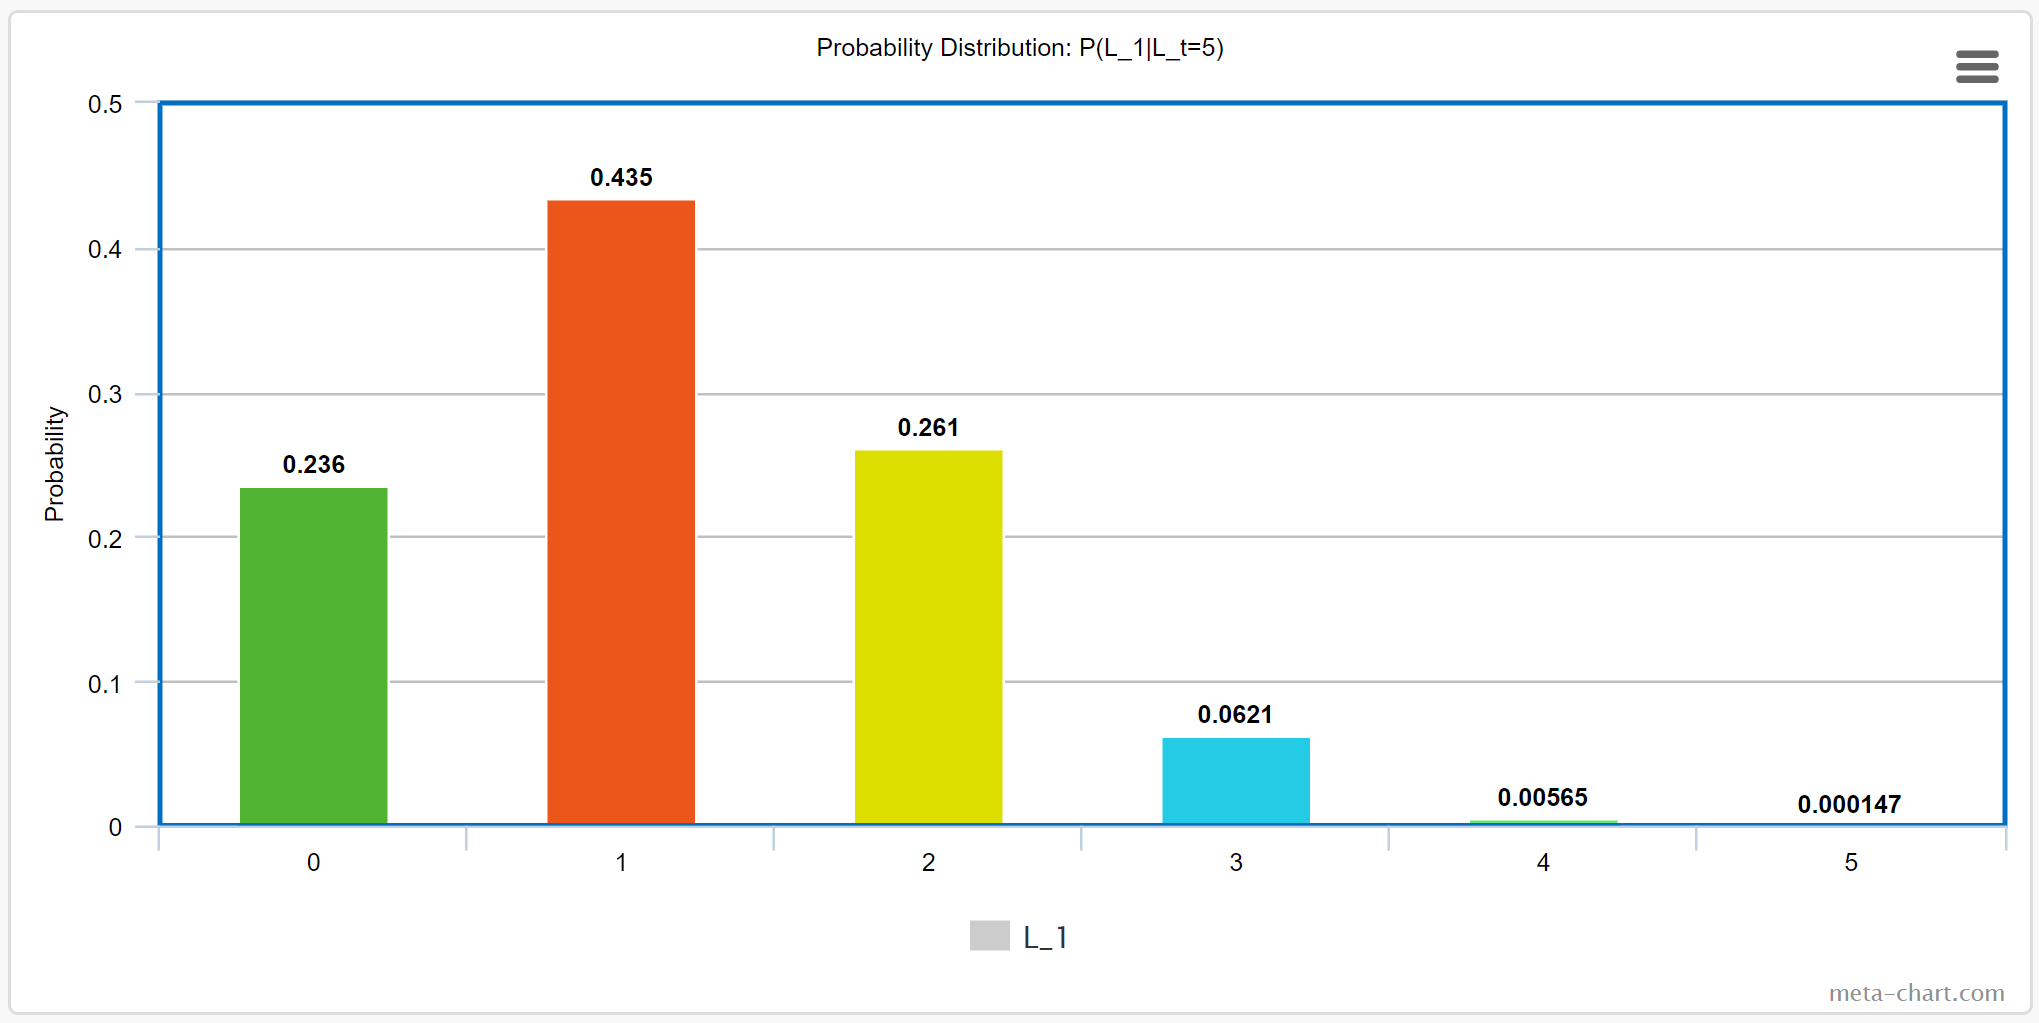
\includegraphics[scale=0.565]{HW4_4.PNG}\newline
 
 \newpage

 \begin{center}
      \Large\textbf{Problem 3:} A continuous random variable has probability density function $\rho(x)$ which is proportional to $g(x)$, where
      \[ 
        g(x)=
        \begin{cases} 
            0 & x < -\frac{\pi}{2} \\
            0 & x > \frac{\pi}{2} \\
            cos(x) & otherwise
        \end{cases}
      \]
      Write c for the constant of proportionality, so that $\rho(x)=cg(x)$.
      \par
 \end{center}

 \textbf{Part A: | What is c? You can look up the integral if you want.}\newline
 
 We must first calculate $\int_{-\infty}^{\infty}g(x)$.
 
 \begin{displaymath}
   \int_{-\infty}^{\frac{-\pi}{2}}g(x) = 
   \int_{-\infty}^{-\frac{\pi}{2}}g(x) + \int_{-\frac{\pi}{2}}^{\frac{\pi}{2}}g(x) + \int_{\frac{\pi}{2}}^{\infty}g(x)
 \end{displaymath}
 
 \begin{displaymath}
   = 0 + 2 + 0 = 2
 \end{displaymath}
  
 By definition, the probability density function must have an integral of 1 from $-\infty$ to $\infty$. Therefore, $\int_{-\infty}^{\infty}\rho(x) = 1$. However, we are given that $\rho(x) = cg(x)$. We can subsequently use the integral we calculated for $g(x)$ earlier to find c. \newline
  
 \begin{displaymath}
    \int_{-\infty}^{\infty}\rho(x)=\int_{-\infty}^{\infty}cg(x)
 \end{displaymath}
 
 \begin{displaymath}
    1=c\int_{-\infty}^{\infty}g(x)
 \end{displaymath}
 
 \begin{displaymath}
    1=c*2
 \end{displaymath}
 
 \begin{displaymath}
    c=\frac{1}{2}
 \end{displaymath}
 
 Final Answer: $c=\frac{1}{2}$.\newline
 
 \textbf{Part B: | What is $P(\{X \geq 0\})$ (i.e. the probability you will observe a value greater than 0)? You can look up the integral if you want.}\newline
 
 By definition, $P(\{X \geq N\})$ of a continuous probability distribution is equal to the following formula: $\int_{N}^{\infty}\rho(x)$, where $\rho(x)$ is the probability density function. We will substitute $0$ for $N$.
 
 \begin{displaymath}
    \int_{0}^{\infty}\rho(x) = \int_{0}^{\infty}\frac{1}{2}g(x)
 \end{displaymath}
 
 \begin{displaymath}
     = \int_{0}^{\frac{\pi}{2}}\frac{1}{2}g(x) + \int_{\frac{\pi}{2}}^{\infty}\frac{1}{2}g(x)
 \end{displaymath}
 
 \begin{displaymath}
     = \int_{0}^{\frac{\pi}{2}}\frac{1}{2}cos(x) + \int_{\frac{\pi}{2}}^{\infty}\frac{1}{2}*0
 \end{displaymath}
 
 \begin{displaymath}
     = \frac{1}{2}
 \end{displaymath}
 
 Final Answer: $\frac{1}{2}$.\newline
 
 \textbf{Part C: |What is $P(\{|X| \leq 1\})$ (i.e. the probability you will observe a value greater than 0)? You can look up the integral if you want.}\newline
 
 We can express $P(\{|X| \leq 1\})$ in the following form: $P(\{-1 \leq X \leq 1\})$. Because this is a continuous probability distribution, we can use an integral to calculate the probability: $\int_{-1}^{1}\rho(x)$, where $rho(x)$ is the probability density function.
 
 \begin{displaymath}
    \int_{-1}^{1}\rho(x) = \int_{-1}^{1}\frac{1}{2}g(x)
 \end{displaymath}
  
 \begin{displaymath}
    = \int_{-1}^{1}\frac{1}{2}cos(x)
 \end{displaymath}
 
 \begin{displaymath}
    = 0.841
 \end{displaymath}
 
 Final Answer: $0.841$.\newline
 
 \newpage
 
 \begin{center}
      \Large\textbf{Problem 4:} Two players P1 and P2 agree to play the following game. Each puts up a stake of 1 unit. They will play seven rounds, where each round involves flipping a fair coin. If the coin comes up H, P1 wins the round, otherwise P2 wins. The first player to win four rounds gets both stakes. After four rounds, P1 has won three rounds and P2 has won one round, but they have to stop. What is the fairest way to divide the stakes?.\par
 \end{center}
 
 Because the game ended early, we will divide up the stakes based on the probability that P1 and P2 wins. Let $x$ be the probability that, should the game continue, player 1 (P1) wins. By definition, $1-x$ is the probability that player 2 (P2) wins. Because there are two stakes, we will give $2x$ stakes to P1 and $2(1-x) = 2-2x$ stakes to P2. In essence, we are giving a larger share of the stakes to the player who has a higher chance of winning the game should the game continue. 
 
 This is similar to distributing 100 pieces of candy to the winner of a basketball game. If the game finishes before four quarters are played, and the first team has a 70\% probability of winning (assume you have psychic statistic abilities and know all probabilities in the world), then the first team gets 70 candies, and the second team gets 30 candies.
 
 Although no clear winner has been established, we are given that P1 has won three rounds and P2 has won one round. Because four rounds have already been played, three rounds remain. In order for P2 to win, he/she must win all three remaining rounds in order to have four wins by the end of the seven rounds. Otherwise, P1 will win. The probability that P2 will win is equal to $\frac{1}{2}*\frac{1}{2}*\frac{1}{2}=\frac{1}{8}$. We can simply multiply together the probabilities that P2 wins rounds 5, 6, and 7, because the events are independent. 
 
 We know that the probability that P1 wins is $1-P(P2$ $ wins)=1-\frac{1}{8}=\frac{7}{8}$, since the two events are mutually exclusive, and either P1 or P2 has to win. Because there is a $\frac{1}{8}$ change that P2 will win, and a $\frac{7}{8}$ chance that P1 will win, we will award $2*\frac{7}{8}=\frac{14}{8}$ units to P1, and $2*\frac{1}{8}=\frac{2}{8}$ units to P2.
 
 Final Answer: P1 gets $\frac{14}{8}$, P2 gets $\frac{2}{8}$.\newline
 
 \newpage
 
 \begin{center}
     \Large\textbf{Problem 5:} An airline company runs a flight that has 10 seats. Each passenger who buys a ticket has a probability p of turning up for the flight. The gender of the passengers is not known until they turn up for a flight, and women buy tickets with the same frequency that men do. The pilot is eccentric, and will not fly unless at least two women turn up (maybe he's an extreme SJW ...)\par
 \end{center}
 
 \textbf{Part A: | How many tickets should the airline sell to ensure that the expected number of passengers that turn up is greater than 10?}\newline
 
 The probability that n passengers will turn up can be calculated using the binomial probability formula because every passenger has an equal probability of showing up. The binomial probability formula can be written as follows:
 
 \begin{displaymath}
    P(x)={n \choose x}p^x(1-p)^{n-x}
 \end{displaymath}
 
 In the above formula, n is the number of trials, x is the number of successful trials desired, and p is the probability that a trial is successful. We can treat each ticket sold as a trial. The trial is successful if the passenger shows up, and unsuccessful if he/she decides to ditch the flight (because who wants to fly on a plane piloted by an SJW)? Ten passengers showing up (aka successes) are desired.
 
 However, we are not trying to calculate the probability that n passengers show up. Instead, we want to calculate n given the fact that 10 passengers must show up. We are simply interested in calculating n given the the expected value is 10; in other words, we want to calculate the number of tickets the airline should sell such that expected number of passengers who show up to be greater than 10. Because the number of passengers who show up is a binomial distribution, we can simply use the formula $E[x]=np$ to calculate the expected number of passengers who show up given $n$ tickets sold and $p$ being the probability that a passenger who buys a ticket shows up. The formula can be derived by finding the expected value of the binomial probability formula written above. Because we want $E[x]$ to be greater than 10, and we already know $p$, we can solve for $n$ using the following formula: $np>10$.
 
 \begin{displaymath}
    np > 10
 \end{displaymath}
 
 \begin{displaymath}
    n > \frac{10}{p}
 \end{displaymath}
 
 Final answer: $n>\frac{10}{p}$\newline
 
 \textbf{Part B: | The airline sells 10 tickets. What is the expected number of passengers on the aircraft, given that it flies? (i.e. that at least two women turn up). Estimate this value with a simulation.}\newline
 
 We used a simulation to get the following graph. We used a numpy seed of 13.\newline
 
 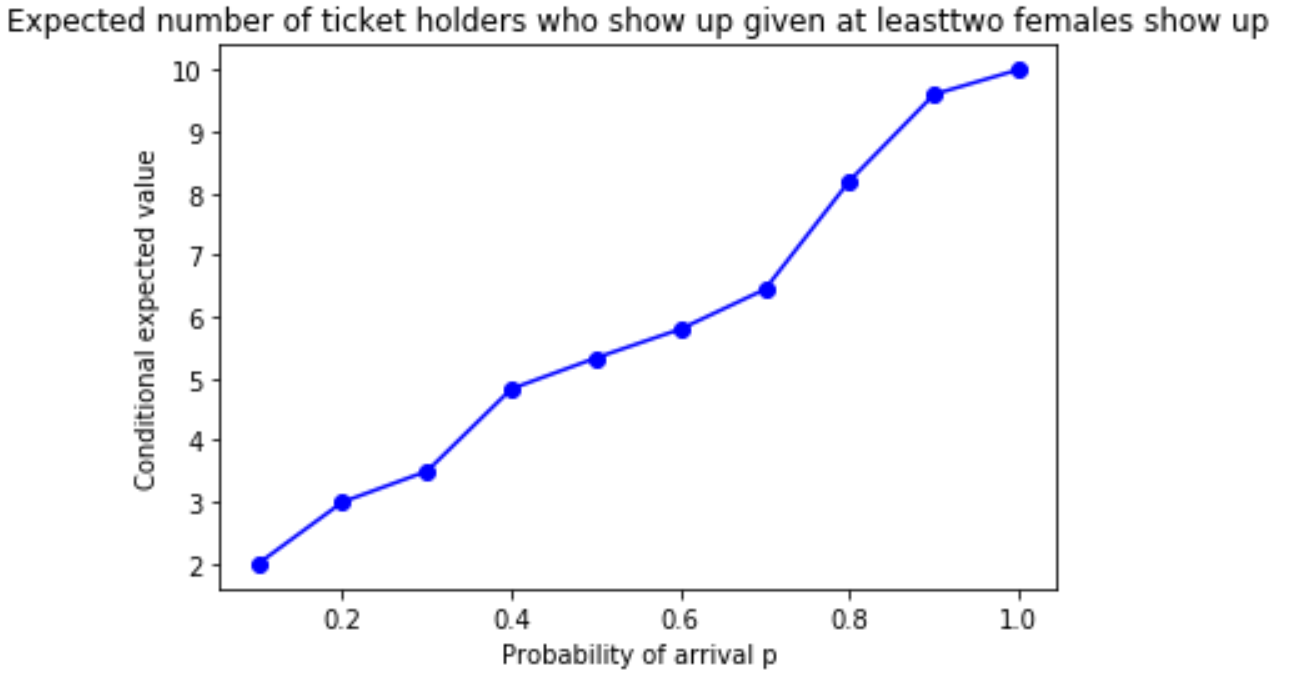
\includegraphics{HW4_5.PNG}
 
 The simulation code is attached to the end of this pdf.\newline
 
 \newpage
 
 \begin{center}
     \Large\textbf{Problem 6:} Show that if X and Y are independent random variables, then $var[X+Y] = var[X] + var[Y]$. You will find it helpful to remember that, for X and Y independent, $E[XY] = E[X]E[Y]$.\par
 \end{center}
 
 \begin{equation}
    var[X+Y] = var[X] + var[Y] + 2*cov(X,Y)
 \end{equation}
 
 The formula for co-variance of two random variables is as follows: $cov(X,Y)=E[XY]-E[X]E[Y]$. We can substitute it into our equation.
 
 \begin{equation}
    var[X+Y] = var[X] + var[Y] + 2*(E[XY]-E[X]E[Y])
 \end{equation}
 
 However, because X and Y are independent, $E[XY]=E[X]E[Y]$. We 
 
 \begin{equation}
    var[X+Y] = var[X] + var[Y] + 2*(E[X]E[Y]-E[X]E[Y])
 \end{equation}
 
 \begin{equation}
    var[X+Y] = var[X] + var[Y] + 2*0
 \end{equation}
 
 \begin{equation}
    var[X+Y] = var[X] + var[Y]
 \end{equation}
 
 Hence, we prove that when X and Y are independent random variables, $var[X+Y]=var[X]+var[Y]$.
 
 \begin{center}
      \Large\textbf{Q.E.D. :)}
 \end{center}
 
 \end{document}

